\documentclass[submit]{harvardml}

% Put in your full name and email address.
\name{Jian Li, Weiyi Chen, Ethan Cowan}
\email{jil761@g.harvard.edu}

% List any people you worked with.
\collaborators{%
Kaggle team - L.C.C.
}

% You don't need to change these.
\course{CS181-S16}
\assignment{Practical \#2}
\duedate{5:00pm March 6th, 2016}

\usepackage[OT1]{fontenc}
\usepackage[colorlinks,citecolor=blue,urlcolor=blue]{hyperref}
\usepackage[pdftex]{graphicx}
\usepackage{subfig}
\usepackage{fullpage}
\usepackage{palatino}
\usepackage{mathpazo}
\usepackage{amsmath}
\usepackage{amssymb}
\usepackage{color}
\usepackage{todonotes}
\usepackage{listings}
\usepackage{common}
\usepackage{bm}

\usepackage[mmddyyyy,hhmmss]{datetime}

\definecolor{verbgray}{gray}{0.9}

\lstnewenvironment{csv}{%
  \lstset{backgroundcolor=\color{verbgray},
  frame=single,
  framerule=0pt,
  basicstyle=\ttfamily,
  columns=fullflexible}}{}

\begin{document}
\begin{center}
{\Large Practical 2: Computer Malware Classification}\\
\end{center}

\section*{1. Introduction}
In this practical we apply machine learning algorithms to the problem of computer malware classification. We have the following $14$ kinds of malware to classify: Agent, AutoRun, FraudLoad, FraudPack, Hupigon, Krap, Lipler, Magania, Poison, Swizzor, Tdss, VB, Virut, and Zbot. Including one additional class of non-malware, we have 15 classes in total. We have 3086 xml files for training and 3724 xml files for testing. Each xml file has a tree-like structure which contains the following layers: processes, process, thread, all sections, and system calls. The system calls are the key input data for malware classification. Each call runs a certain command such as 'load image' or 'load dll' with keyed attributes such as filename or size. The Python xml ElementTree library is used here to navigate the xml tree structure and extract system calls.
$x$

The rest of the report is organized as follows: we start by explaining how we extract features and how we decide the importance of features, followed by the detailed analysis of testing different types of algorithms including Random Forest, Extra Random Tree, and Support Vector Machine. The last section conclude the report with our best score on Kaggle.
\section*{2. Feature Extraction}
We think of the following features to extract from the xml files:
\begin{enumerate}
\item The number of each type of system call in the xml file.
\item The structure of the system calls within the file.
\item The attributes of each call.
\end{enumerate}
For the first feature, we first run through all training samples and determine the universe of system calls appearing in the file, excluding the four structural tags: processes, process, thread, and all section. We get 102 distinct system calls in the universe and then count the number of times each of them is called in the training set and testing set, and use this 102 dimension vector as our feature. 

We divided the training samples into two subsets of 1543 samples. The first half is used for fitting while the second half is used for validation. This way we can quickly test the in-sample and out-of-sample error. The split of the subset is based on alphabetical ordering of the files so it doesn't guarantee each class will have the same percentage of samples. As a result, there's a slight bias of class distribution between the fitting set and the full training set but it is small - less than $0.58\%$ for each class.

We use a Random Forest(RF) classifier to determine the relative importance of each feature. The feature importance scores after training shows that 78 out of 102 features have non-zero scores. When we throw away the other 24 features, the out-of-sample classification error goes down slightly, so we keep those features in most of our experiments.

Our base line classifier is a RF classifier with number of estimators 30, max features 30, and minimum samples of split 4. The next section will show details of how we picked these parameters. This base classifier has $2.1\%$ in-sample error rate and $11.4\%$ out-of-sample error rate. This error rate varies slightly in each run due to the random nature of RF classifier but it is within a close range.

We tried a couple of other approaches with this feature vector. First we mapped the feature vector to a binary scheme by using 1 for each feature when there is at least one such system call and zero otherwise. The performance drops to $3.8\%$ and $12.6\%$ for in-sample and out-of-sample errors. The second approach is to normalize the feature vector by the total number of calls in each xml file, which has better in-sample rate of $1.9\%$ but worse out-of-sample rate of $11.8\%$. So the original feature vector perform better than both binary and normalized vectors and we used them in our tests unless otherwise noted.

For the second feature on the list, the structure refers to the nesting of different calls within a process or a thread, and the ordering of the calls. The combination of grouping or ordering different calls is large and may not be suitable for this problem with only 3086 training samples. Some prior knowledge about different types of malware will help us to decide which part of xml tree is more relevant. The third feature looks at different attributes used for each call and can be an important feature for different types of malware. It's tricky to pick out which attribute to use and how to standardize string input such as filename. Due to the time constraint, we did not extract features in this category.

\section*{3. Methods Description and Results Discussion}
We started with multiple classes of algorithms: linear models, neighbors, naive bayes, ensemble methods and SVM. Given the rough results, we concentrated on several tested algorithms and describe our motivations to continue our optimization on these methods: Random Forest (RF), Extra Random Tree (ET), and Support Vector Machine (SVM).

\subsection*{3.1 General}

We simply took features described above to train the classifier and used the classifier to predict given test data's features. Based on our experience from practical 1 that the difference between different methods in the same class is comparably small, compared to the difference between different classes. Below is the result of several representative methods from multiple classes -

\begin{center}
  \begin{tabular}{ | l | l | }
    \hline
    Method & Kaggle Public Score \\ \hline
    Linear methods & $54.26\%$ \\ \hline
    Naive Bayes & $60.68\%$ \\ \hline
    Neighbor methods & $74.05\%$ \\ \hline
    Ensemble methods &  $79.53\%$ \\ \hline
    Tree methods & $78.52\%$ \\ \hline        
    SVM & $70.63\%$ \\ \hline               
  \end{tabular}
\end{center}

We can see ensemble methods, tree methods and SVM perform better than other kinds of methods. Motivated from this, we continue our research on these methods and dig into feature importance to optimize.

\subsection*{3.2 Random Forest Classification}
RF is a popular ensemble method that use various sub-sets of the dataset then combines weak classifiers such as binary decision tree to improve accuracy and reduce overfitting. It has three main parameters to test: number of estimators, max features which is the number of features to consider when looking for the best split, and the minimum number of samples required to split an internal node.  

We use cross validation to test a range of values for these three parameters: number of estimators from 10 to 200, max features from 5 to 102, and number of minimum sample split from 1 to 50. The out-of-sample error rate is used to evaluate the quality of each classifier. Although each run of RF produces slightly different results, the best parameters we found are: number of estimators 30, max features 10 or 30, and min sample split 4, with out-of-sample error rate around $11.79\%$ and $11.40\%$.

We also put together the following misclassification matrix to analyze the difficulty of separating each pair of classes. In Figure \ref{fig:rf_in} and \ref{fig:rf_out} we show in-sample and out-of-sample misclassifications. Each row shows the correct class label, and each column shows the incorrect class a sample has been misclassified to. The graph gives the number of misclassified samples out of the total of 1543 samples in the training set for in-sample error, and the one in the validation set for out-of-sample error. We put a heat map on these numbers. As the most commonly seen misclassifications are Agent, VB, and Virut misclassified as None - not a malware. This tells us that future improvements should focus on the difference between these three and the None class.

\begin{figure}[htbp]
\centering
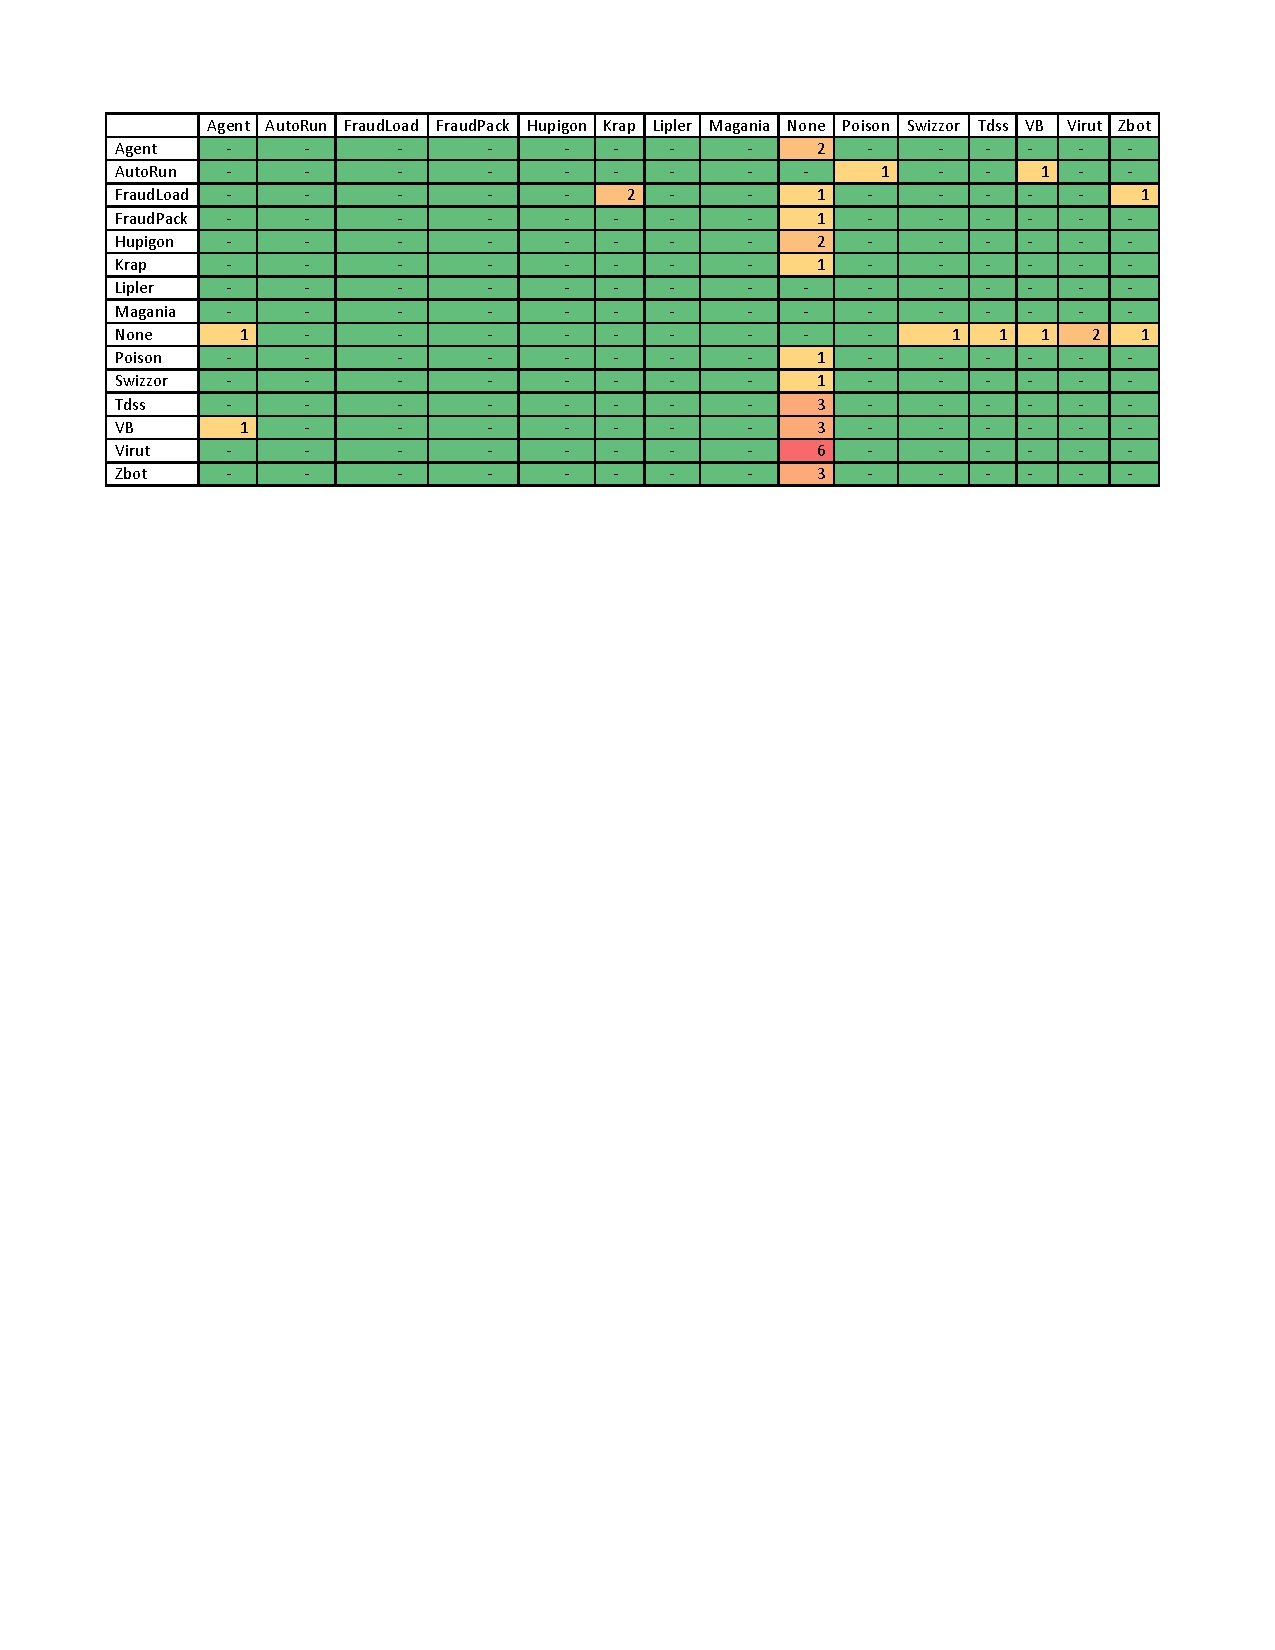
\includegraphics[width=0.95\textwidth]{RF_in}
\caption{Random Forest in-sample misclassification pattern.}
\label{fig:rf_in}
\end{figure}

\begin{figure}[htbp]
\centering
%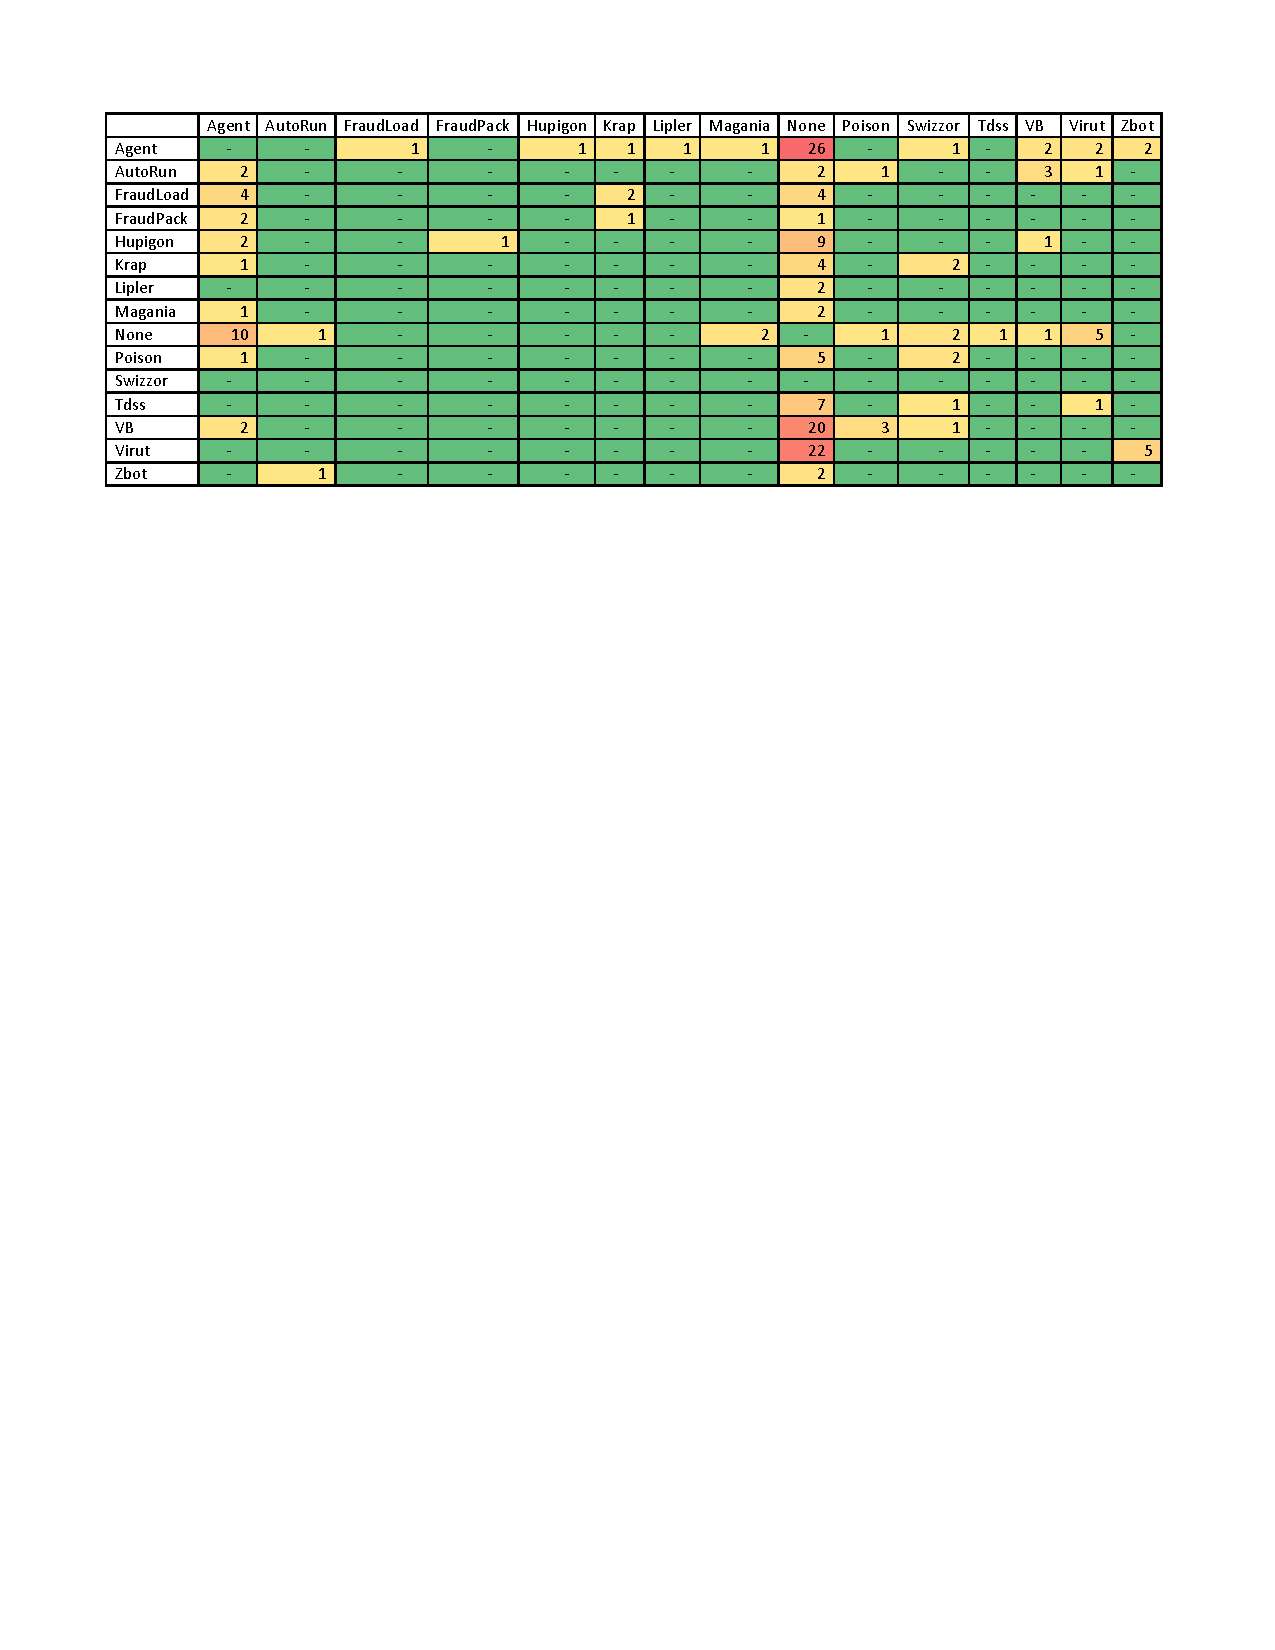
\includegraphics[clip, trim=0.5cm 11cm 0.5cm 11cm, width=1.00\textwidth]{RF_out}
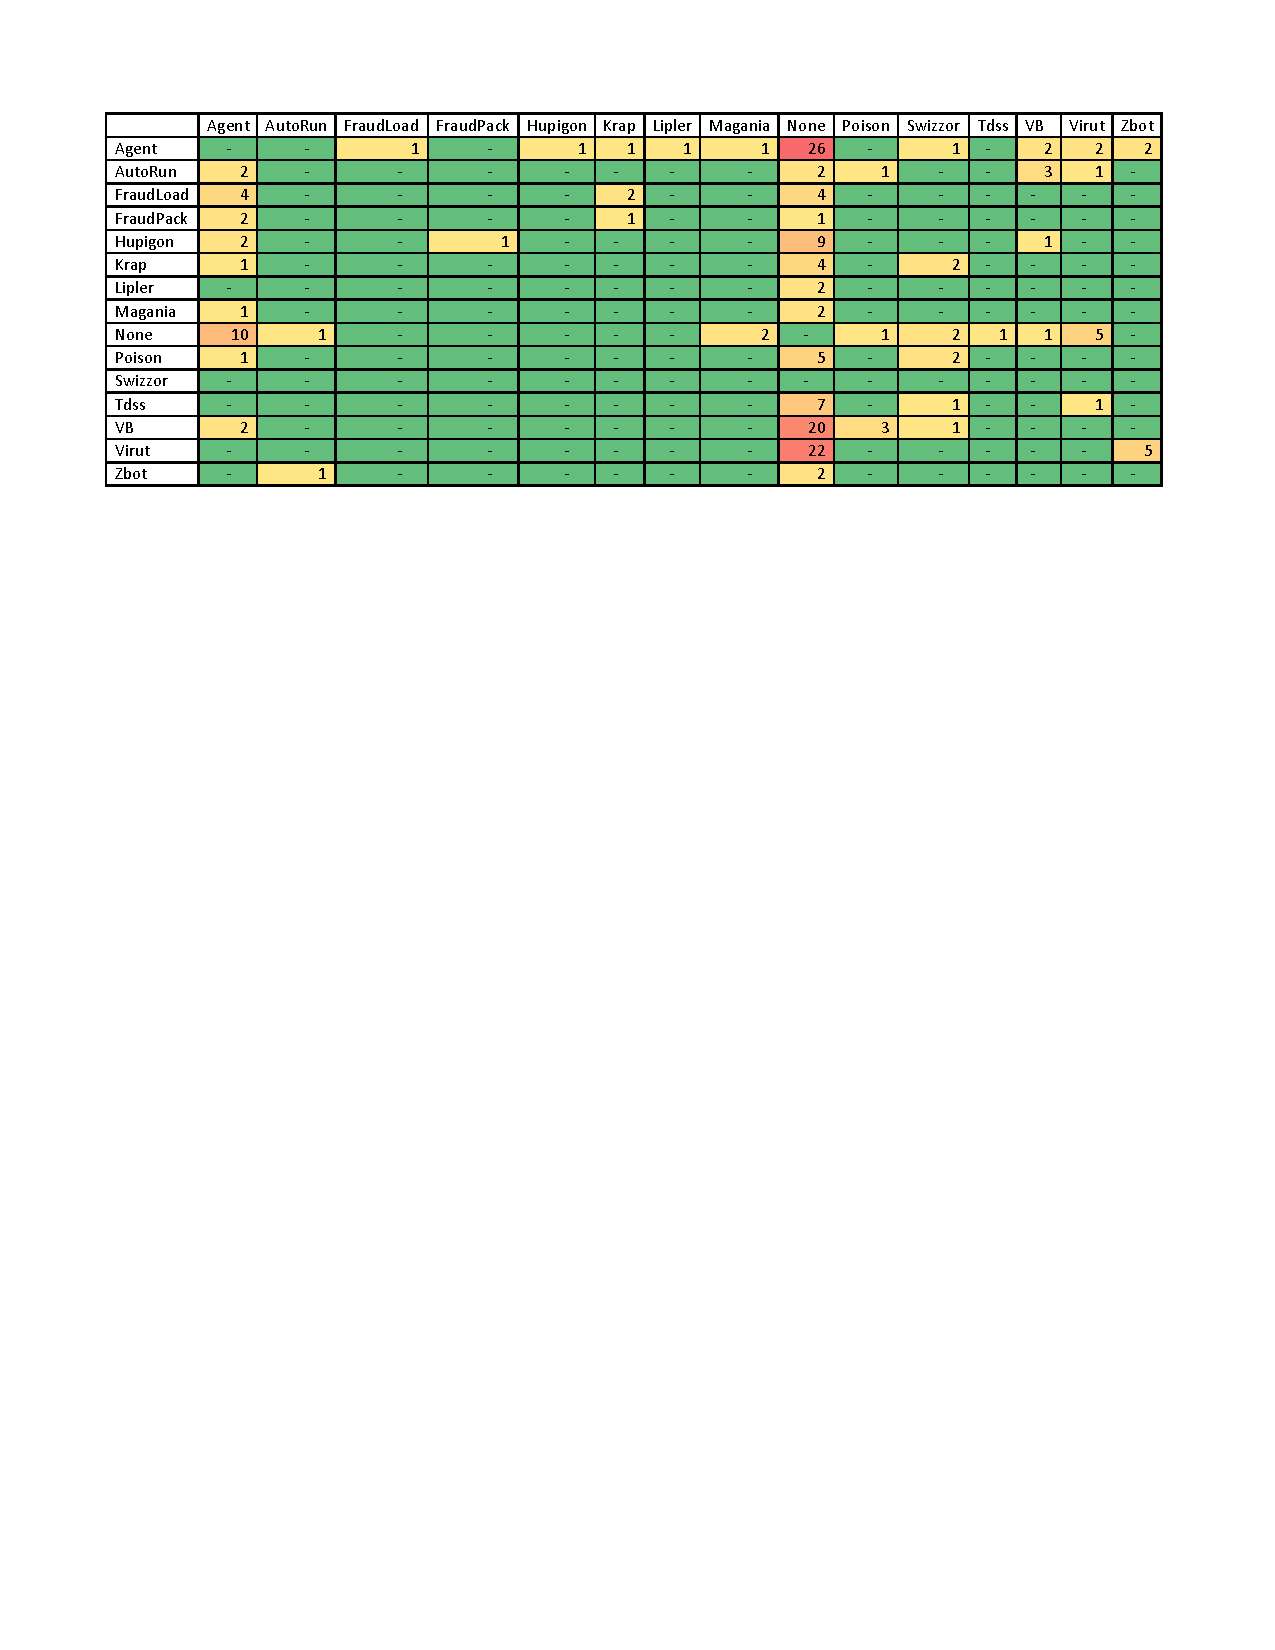
\includegraphics[width=0.95\textwidth]{RF_out}
\caption{Random Forest out-of-sample misclassification pattern.}
\label{fig:rf_out}
\end{figure}

\subsection*{3.3 Extra Random Tree Classification}
This method is also called Extremely Randomized trees. Additional randomness is added compared to RF during the process of selecting thresholds for randomly selected features to compute further splits of the decision tree. While in RF, the most discriminative thresholds are calculated, in ET, these thresholds are drawn at random. ET usually has the advantage of futher reducing variance, at the expense of increasing bias.

The three key parameters are the same as RF classifier. We again test a range of values and use cross validation to determine the best parameters. The result is the same as RF with number of estimators 30, max features 10, and minimum sample split 4. The in-sample error rate is $1.88\%$ and the out-of-sample error rate is $11.02\%$, so slightly improved over RF.

\subsection*{3.4 Support Vector Machine}

SVM, a max margin based approach for classification, is a robust classifier because it tries to maximize the distance of classification boundaries. The kernel trick can also be applied to SVM to map the features to a higher dimensional space implicitly. 

Here we tested the default version of SVC (SVM classifier) in the sklearn package, with RBF as kernel function and C chosen as 1.0 (the weighting of the error term). We get in-sample error of $4.34\%$ and out-of-sample error of $23.84\%$, with both much higher than RF and ET methods. 

In order to improve results, we ran extensive testing in the following parameters:
\begin{enumerate}
\item Kernel and degree: we tested RBF kernel, polynomial kernel, and sigmoid kernel. The sigmoid kernel gives significant error here so we focus on the first two kernels. For polynomial kernels, we tested degree 2 and 3.
\item C: This parameter controls the weighting of the error term. When C is large, we penalize more of misclassification, at the cost of reducing the margin and making the classifier less robust. 
\item gamma: gamma is the coefficient inside the kernel. By default it's set to 1/number of features.
\item coef$_0$: a bias item used in the polynomial kernel calculation. In the tests we observe setting coef$_0$ to zero gives the best results.
\end{enumerate}

Here we focus on three types of kernels and find the best parameters for each: RBF, polynomial with degree 2, and polynomial with degree 3. Polynomial kernel with degree 2 gives the best validation results at $15.16\%$. In the actual Kaggle score, RBF gives the best results. The results of validation for parameter selection is summarized in the table below.

\begin{center}
  \begin{tabular}{ | l | l | l | l | }
    \hline
    Kernel & Parameters & In-sample error & Out-of-sample error \\ \hline
    RBF & C=10,gamma= 1/(35 * number of features) & $6.74\%$ & $17.69\%$ \\ \hline
		Polynomial, degree 2 & C=0.01,gamma= 1/(2 * number of features)  & $7.12\%$ & $15.16\%$ \\ \hline
		Polynomial, degree 3 &  C=0.0001,gamma= 1/number of features & $6.66\%$ & $16.52\%$ \\ \hline
  \end{tabular}
\end{center}

\section*{4. Conclusion}
Our Kaggle team name is L.C.C.. Our Kaggle submissions are listed below. The best score is $81.21\%$ for RF with 102 features, 30 estimators, 10 max features, and 4 minimum sample split. The 61 features used are the most important features based on the RF classification results.

We can see the advantage of RF being that it doesn't have many parameters to tune so it is easy to train and fast to run. SVM gives many options of kernels and parameters but it takes many run to pick the optimal parameters for each problem. In this case its performance is not as good as RF.

\begin{center}
  \begin{tabular}{ | l | l | l | }
    \hline
    Method & Parameters & Kaggle Public Score \\ \hline
    Random Forest & 102 features, 30 estimators, 10 max features, 4 min samples split & $81.21\%$ \\ \hline
		Extra Random Trees & 102 features, 30 estimators, 10 max features, 4 min samples split & $80.52\%$ \\ \hline				
		    Extra Random Trees & 61 features, 30 estimators, 10 max features, 4 min samples split & $80.21\%$ \\ \hline
				    Random Forest & 61 features, 30 estimators, 10 max features, 4 min samples split & $79.68\%$ \\ \hline
						    Random Forest & 102 features, 30 estimators, 30 max features, 4 min samples split & $79.53\%$ \\ \hline
SVM RBF Kernel & C=10,gamma= 1/(35 * number of features) & $75.11\%$ \\ \hline
SVM Polynomial Kernel & C=0.01,degree=2,gamma= 1/(2 * number of features) & $71.58\%$ \\ \hline
SVM Polynomial Kernel & C=0.0001,degree=3,gamma= 1/number of features & $70.63\%$ \\ \hline								
  \end{tabular}
\end{center}

\end{document}
